\subsection{MVC 模式}

MVC模式(Model-View-Controller pattern)是一种用于分离应用程序的数据模型(Model)、用户界面(View)和业务逻辑(Controller)的设计模式。

在MVC模式中,Model代表应用程序的数据模型,它负责处理与数据相关的业务逻辑,例如对数据进行验证、查询和修改等。View代表用户界面,它负责显示数据和与用户交互,例如显示表单和按钮等。Controller负责接收用户的请求,并调用Model和View来完成相应的业务逻辑和显示数据。

使用MVC模式的主要目的是将应用程序的业务逻辑和用户界面进行分离,使得两者之间的耦合度降到最低。这样,如果需要更改用户界面或业务逻辑,只需要修改相应的View或Controller即可,而不需要修改整个应用程序。

MVC模式通常用于构建大型的,复杂的应用程序,例如企业应用程序或Web应用程序。它可以帮助开发人员更轻松地处理应用程序的业务逻辑和用户界面,并使应用程序更容易维护和扩展。

\begin{figure}[htb]
  \centering
  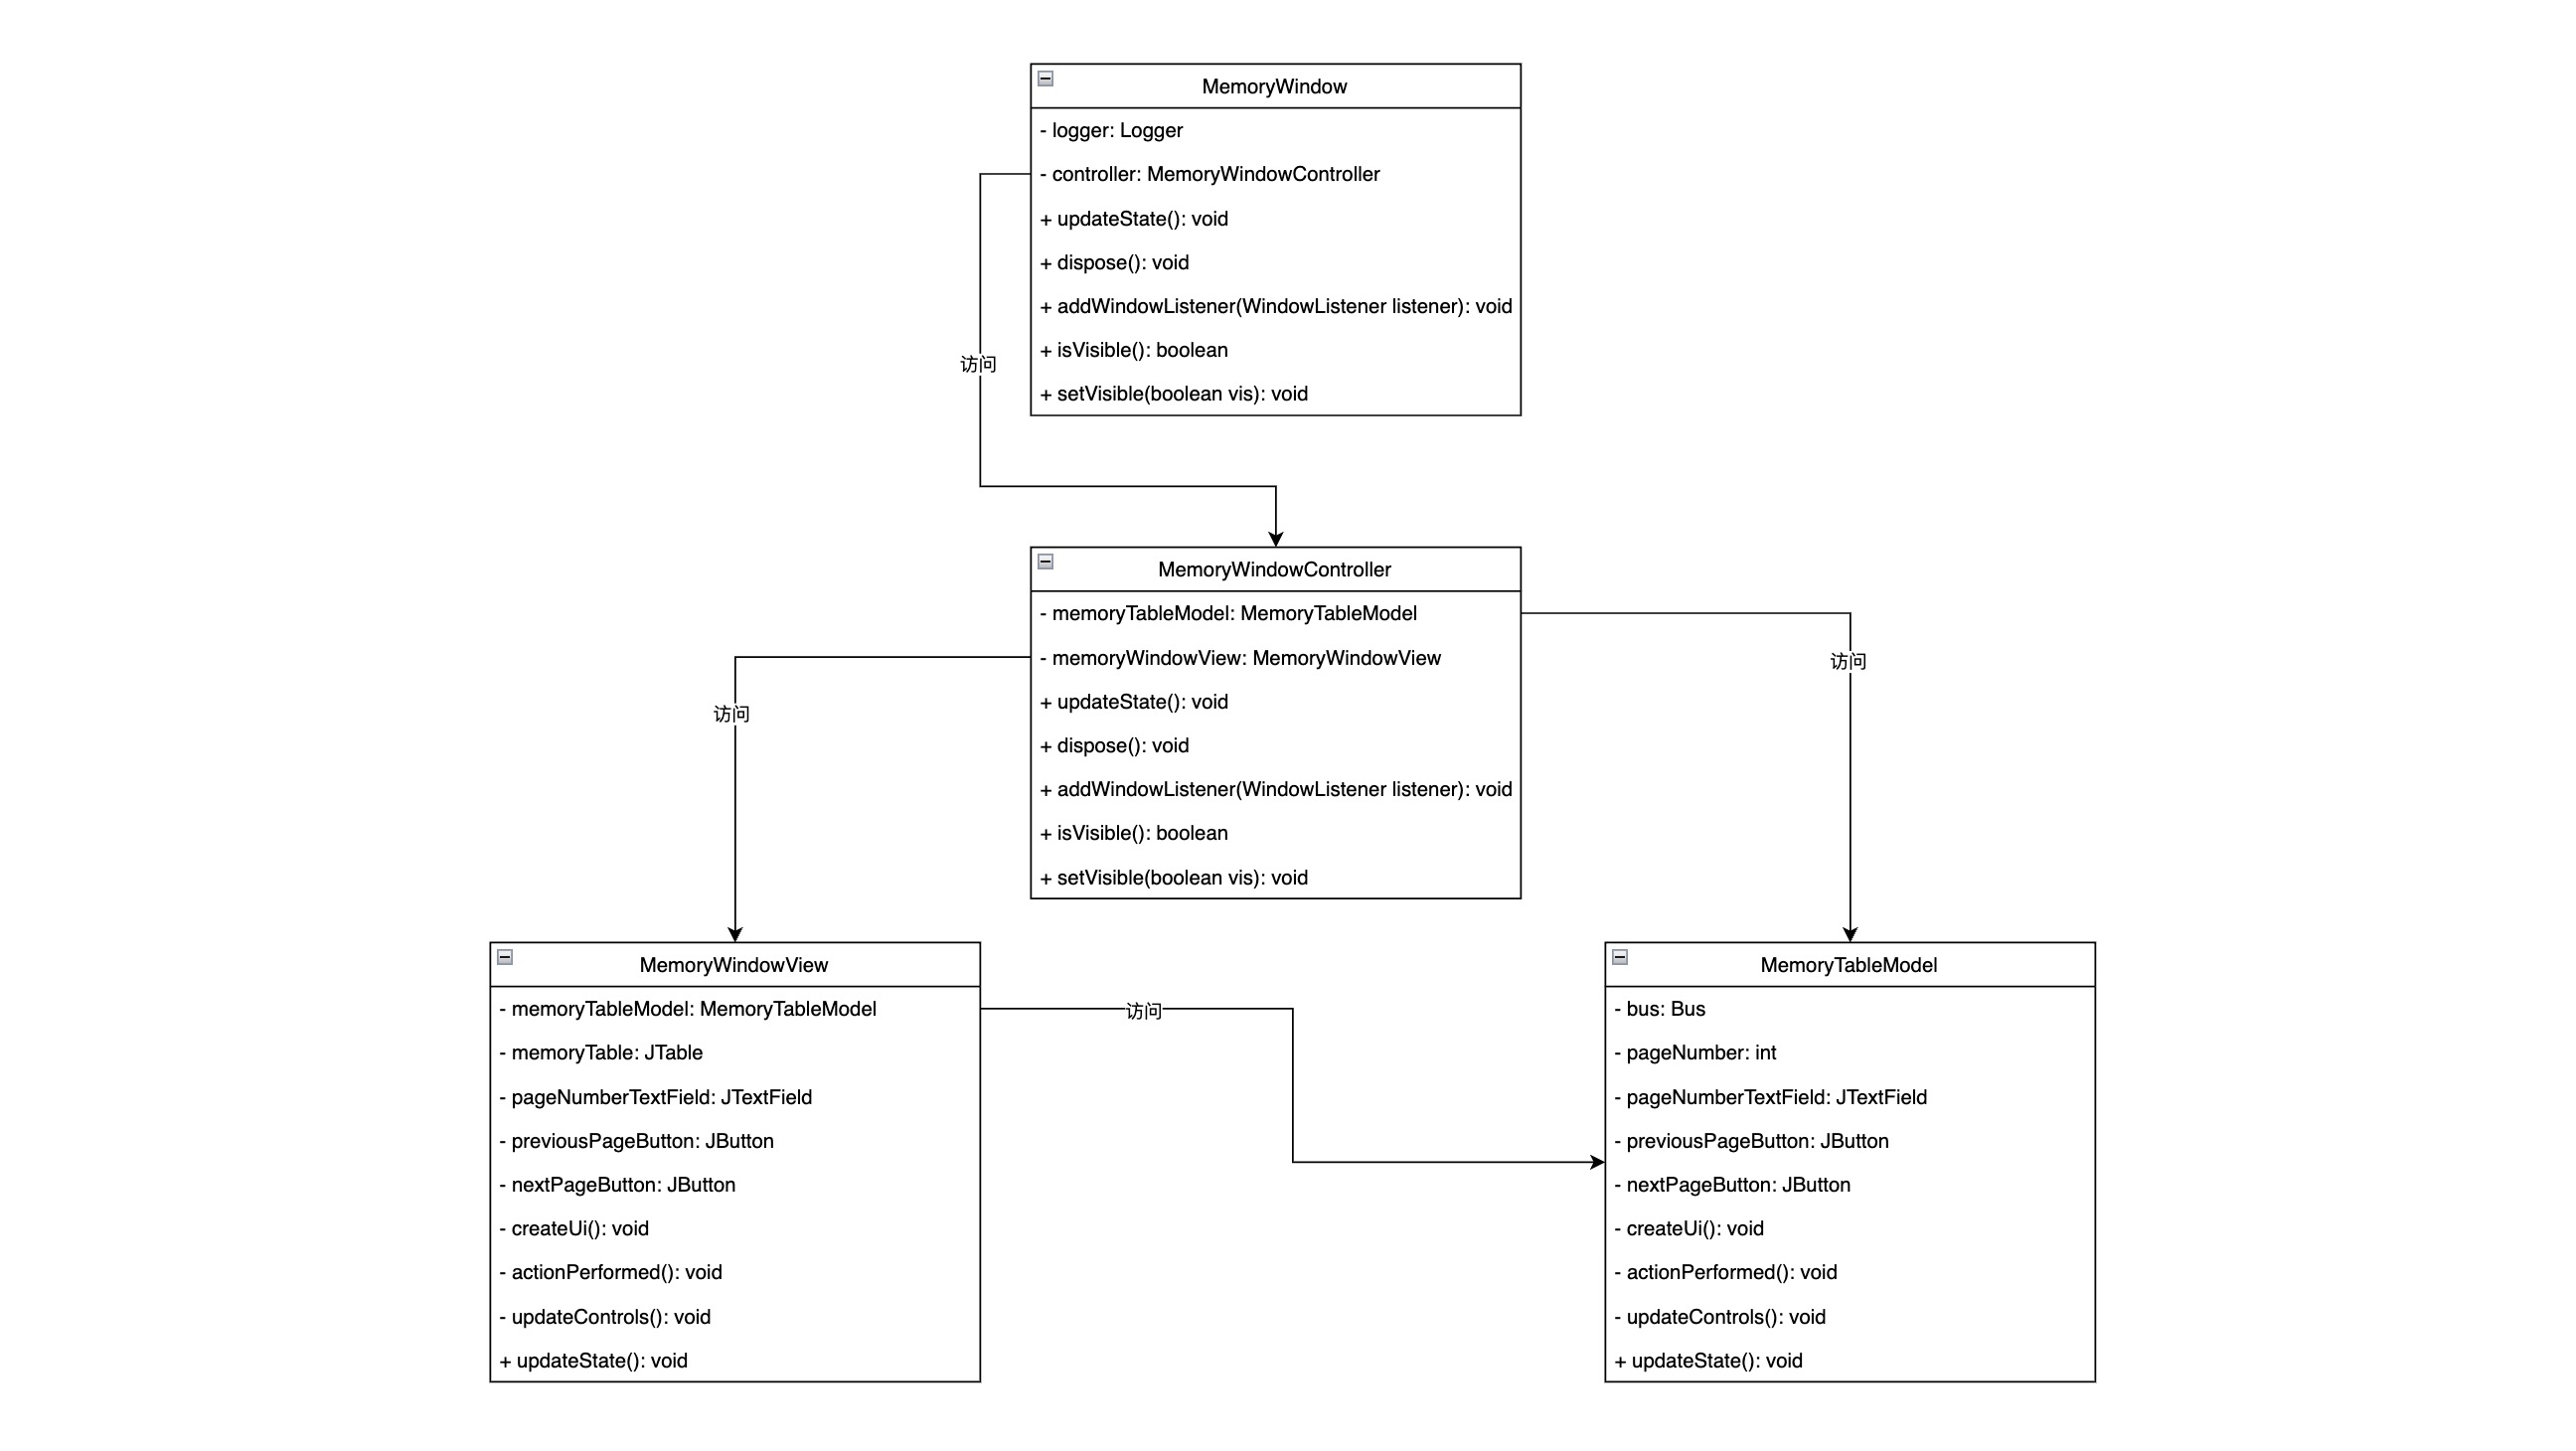
\includegraphics[width=0.9\textwidth]{figures/MVC模式.jpg}
  \caption{MVC 模式在 Slow6502 中的类图}
\end{figure}

在MemoryWindow页面使用MVC模式,使得逻辑控制、组件UI实现、数据模型处理逻辑分离,能够使得前端整体架构更加解耦。控制器的职责是接收用户的输入并将其转发给模型,然后根据模型的响应更新视图。

